% -*- TeX-master: "sbml-level-3-version-1-core"; fill-column: 66 -*-
% $Id$
% $HeadURL$
% ----------------------------------------------------------------

\section{The Systems Biology Ontology and the \token{sboTerm} attribute}
\label{sec:sboTerm}
\label{sec:sbo}

The values of \token{id} attributes on SBML components allow the
components to be cross-referenced within a model. The values of
\token{name} attributes on SBML components provide the opportunity
to assign them meaningful labels suitable for display to humans
(Section~\ref{sec:idnameattribs}).  The specific identifiers and
labels used in a model necessarily must be unrestricted by SBML,
so that software and users are free to pick whatever they need.
However, this freedom makes it more difficult for software tools
to determine, without additional human intervention, the semantics
of models more precisely than the semantics provided by the SBML
object classes defined in other sections of this document.  For
example, there is nothing inherent in a parameter with identifier
``\token{k}'' that would indicate to a software tool it is a
first-order rate constant (if that's what ``\token{k}'' happened
to be in some given model).  However, one may need to convert a
model between different representations (\eg
Henri-Michaelis-Menten vs.\ elementary steps), or to use it with
different modeling approaches (discrete or continuous).  One may
also need to relate the model components with other description
formats such as SBGN (\url{http://www.sbgn.org/}) using deeper
semantics.  Although an advanced software tool \emph{might} be
able to deduce the semantics of some model components through
detailed analysis of the kinetic rate expressions and other parts
of the model, this quickly becomes infeasible for any but the
simplest of models.

An approach to solving this problem is to associate model
components with terms from carefully curated controlled
vocabularies (CVs).  This is the purpose of the optional
\token{sboTerm} attribute provided on the SBML
class \SBase.  The \token{sboTerm} attribute always refers to
terms belonging to the Systems Biology Ontology (SBO, \sboref). In
this section, we discuss the \token{sboTerm} attribute,
SBO, the motivations and theory behind their introduction, and
guidelines for their use.

SBO is not part of SBML; it is being developed separately, to
allow the modeling community to evolve the ontology independently
of SBML.  However, the terms in the ontology are being designed
keeping SBML components in mind, and are classified into subsets that
can be directly related with SBML components such as reaction rate
expressions, parameters, and a few others, see below.  The use of
\token{sboTerm} attributes is optional, and the presence of
\token{sboTerm} on an element does not change the way the model is
\emph{interpreted}.  Annotating SBML elements with SBO terms
adds additional semantic information that may be used to
\emph{convert} the model into another model, or another format.
Although SBO support provides an important source of information to
understand the meaning of a model, software does not need to
support \token{sboTerm} to be considered SBML-compliant.

\subsection{Principles}
\label{sec:sbo-principles}

Labeling model components with terms from shared controlled
vocabularies allows a software tool to identify each component using
identifiers that are not tool-specific.  An example of where this
is useful is the desire by many software developers to provide
users with meaningful names for reaction rate equations.  Software
tools with editing interfaces frequently provide these names
in menus or lists of choices for users.  However, without a
standardized set of names or identifiers shared between
developers, a given software package cannot reliably interpret the
names or identifiers of reactions used in models written
by other tools.

The first solution that might come to mind is to stipulate that
certain common reactions always have the same name (\eg
``Michaelis-Menten''), but this is simply impossible to do: not
only do humans often disagree on the names themselves, but it
would not allow for correction of errors or updates to the list of
predefined names except by issuing new releases of the SBML
specification---to say nothing of many other limitations with this
approach.  Moreover, the parameters and variables that appear in
rate expressions also need to be identified in a way that software
tools can interpret mechanically, implying that the names of these
entities would also need to be regulated.

The Systems Biology Ontology (SBO) provides terms for identifying
most elements of SBML.  The relationship implied by an
\token{sboTerm} on an SBML model component is ``is-a'' between the
characteristic of the component meant to be described by SBO on
this element and the SBO term identified by the value of the
\token{sboTerm}.  By adding SBO term references on the components
of a model, a software tool can provide additional details using
shared vocabularies that can enable \emph{other} software tools to
recognize precisely what the component is meant to be.  Those
tools can then act on that information.  For example, if the SBO
identifier \token{SBO:0000049} is assigned to the concept of
``first-order irreversible mass-action kinetics, continuous
framework'', and a given \KineticLaw object in a model has an
\token{sboTerm} attribute with this value, then regardless of the
identifier and name given to the reaction itself, a software tool
could use this to inform users that the reaction is a first-order
irreversible mass-action reaction.  This kind of reverse
engineering of the meaning of reactions in a model would be
difficult to do otherwise, especially for more complex reaction
types.

The presence of SBO labels on \Compartment, \Species, and
\Reaction objects in SBML can help map those entities to
equivalent concepts in other standards, such as (but not limited
to) BioPAX (\url{http://www.biopax.org/}), PSI-MI
(\url{http://www.psidev.info/index.php?q=node/60}), or the Systems
Biology Graphical Notation (SBGN, \url{http://www.sbgn.org/}).
Such mappings can be used in conversion procedures, or to build
interfaces, with SBO becoming a kind of ``glue'' between standards
of representation.

The presence of the label on a kinetic expression can also allow
software tools to make more intelligent decisions about reaction
rate expressions.  For example, an application could recognize
certain types of reaction formulas as being ones it
knows how to solve with optimized procedures.  The application
could then use internal, optimized code implementing the rate
formula indexed by identifiers such as \token{SBO:0000049}
(``mass action rate law for first order irreversible reactions,
continuous scheme'') appearing in SBML models.

Finally, SBO labels may be very valuable when it comes to model
integration, by helping identify interfaces, convert mathematical
expressions and parameters etc.

Although the use of SBO can be beneficial, it is critical to keep
in mind that the presence of an \token{sboTerm} value on an object
\emph{must not change the fundamental mathematical meaning} of the
model.  An SBML model must be defined such that it stands on its
own and does not depend on additional information added by SBO
terms for a correct mathematical interpretation.  SBO term
definitions will not imply any alternative mathematical semantics
for any SBML object labeled with that term.  Two important
reasons motivate this principle.  First, it would be too limiting
to require all software tools to be able to understand the SBO
vocabularies in addition to understanding SBML.
Supporting SBO is not only additional work for the software
developer; for some kinds of applications, it may not make sense.
If SBO terms on a model are optional, it follows that the SBML
model \emph{must} remain unambiguous and fully interpretable
without them, because an application reading the model may ignore
the terms.  Second, we believe allowing the use of \token{sboTerm}
to alter the mathematical meaning of a model would allow
  too much leeway to shoehorn inconsistent concepts into SBML
objects, ultimately reducing the interoperability of the
models.

\subsection{Using SBO and \token{sboTerm}}

The \token{sboTerm} attribute data type is always
\primtype{SBOTerm}, defined in Section~\ref{sec:sboterm-type}.
When present in a given model object instance, the
attribute's value must be an identifier taken from the
Systems Biology Ontology (SBO; \sboref).  This identifier must
refer to a single SBO term that best defines the entity encoded by
the SBML object in question.  An example of the type of
relationship intended is: \emph{the KineticLaw in reaction R1 is a
  first-order irreversible mass action rate law}.

Note the careful use of the words ``defines'' and ``entity encoded
by the SBML object'' in the paragraph above.  As mentioned, the
relationship between the SBML object and the URI is:

\begin{quote}
  The ``thing'' encoded by this SBML object has a characteristic
  that is an instance of the ``thing'' represented by the
  referenced SBO term.
\end{quote}

The characteristic relevant for each SBML object is described in
the second column of Table~\ref{tab:sboterm-availability}.


\subsubsection{The structure of the Systems Biology Ontology}

The goal of SBO labeling for SBML is to clarify to the fullest
possible extent the nature of each element in a model.  The
approach taken in the Systems Biology Ontology begins with a
hierarchically-structured set of controlled vocabularies with six
main divisions: (1) entity, (2) participant role, (3) quantitative
parameter, (4) modeling framework, (5) mathematical expression,
and (6) interaction.  Figure~\vref{fig:sbo-top-level} illustrates
the highest level of SBO.

Each of the six branches of Figure~\ref{fig:sbo-top-level} has a
hierarchy of terms underneath them.  At this time, we can only
begin to list some initial concepts and terms in SBO; what follows
is not meant to be complete, comprehensive or even necessarily
consistent with future versions of SBO.  The web site for SBO
(\sboref) should be consulted for the current version of the
ontology.  Section~\ref{sec:sbo-frequency-of-change} describes how
the impact of SBO changes on software applications is minimized.

\begin{figure}[tbh]
  \centering
  
\includegraphics[scale = 0.8]{figs/sbo-top-level}
  \vspace*{1ex}
  \caption{The six controlled vocabularies (CVs) that
      make up the main branches of SBO.}
  \label{fig:sbo-top-level}
\end{figure}

Figure~\vref{fig:expanded-species} shows the structure for the
\emph{entity} branch, which reflects the hierarchical groupings of
the types of entities that can be represented by a \Compartment or
\Species object.  Note that the values taken by the
\token{sboTerm} attribute on those elements should refer to SBO
terms belonging to the \emph{material entity} branch, so as to
distinguish whether the element represents a macromolecule, a
simple chemical, etc.  Indeed, this information remains valid for
the whole model. The term should not belong to the
\emph{functional entity} branch, representing the function of the
entity within a certain functional context. If one wants to use
this information, one should refer to the SBO terms using a
controlled RDF annotation instead
(Section~\ref{sec:annotation-standard}), carefully choosing the
qualifiers (Section~\ref{sec:qualified-dc-annotation}) to reflect
the fact that a given \Species object, for instance, can fulfill
different functions within a given model (\eg EGF receptor is a
receptor and an enzyme).

\begin{figure}[htb]
  \centering
  \vspace*{-1ex}
  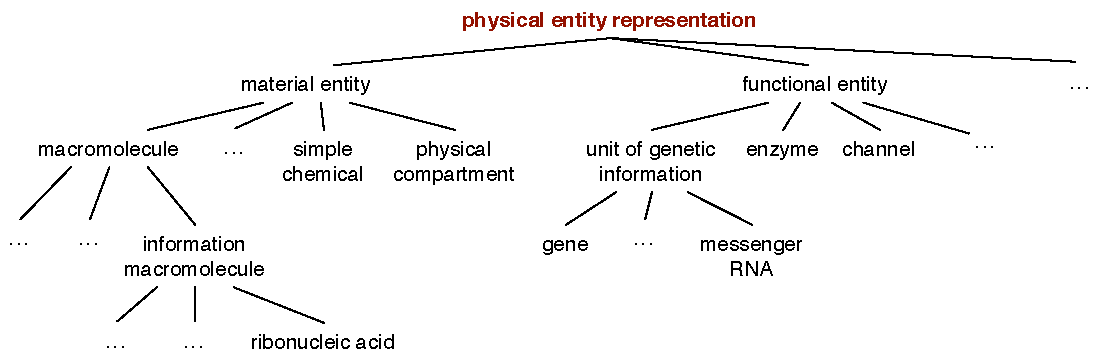
\includegraphics[scale = 0.78]{figs/sbo-entity}
  \caption{Partial expansion of some of the terms in the
    \emph{entity} branch of SBO.}
  \label{fig:expanded-species}
\end{figure}

Figure~\vref{fig:expanded-speciesRef} shows the structure for the
\emph{participant role} branch, also grouping the concepts in a
hierarchical manner.  For example, in reaction rate expressions,
there are a variety of possible modifiers.  Some classes of
modifiers can be further subdivided and grouped.  All of this is
easy to capture in the ontology.  As more agreement is reached in
the modeling community about how to define and name modifiers for
different cases, the ontology can grow to accommodate it.

\begin{figure}[htb]
  \centering
  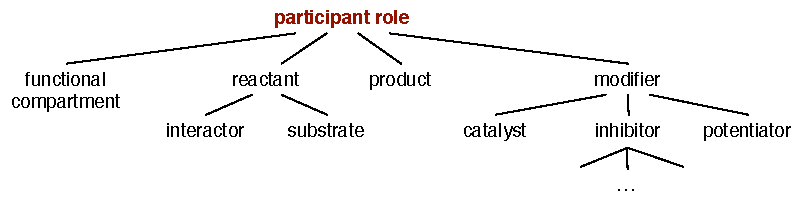
\includegraphics[scale = 0.87]{figs/sbo-participant-role}
  \caption{Partial expansion of some of the terms in the
    \emph{participant role} branch of SBO.}
  \label{fig:expanded-speciesRef}
\end{figure}

The controlled vocabulary for quantitative parameters is
illustrated in Figure~\vref{fig:expanded-parameter}.  Note the
separation of \emph{kinetic constant} into separate terms for
unimolecular, bimolecular, etc. reactions, as well as for forward
and reverse reactions.  The need to have separate terms for
forward and reverse rate constants arises in reversible
mass-action reactions.  This distinction is not always necessary
for all quantitative parameters; for example, there is no
comparable concept for the Michaelis constant.  Another
distinction for some quantitative parameters is decomposition into
different versions based on the modeling framework being assumed.
For example, different terms for continuous and discrete
formulations of kinetic constants represent specializations of the
constants for particular simulation frameworks.  Not all
quantitative parameters will need to be distinguished along this
dimension.

\begin{figure}[tbh]
  \centering
  \vspace{-2ex}
  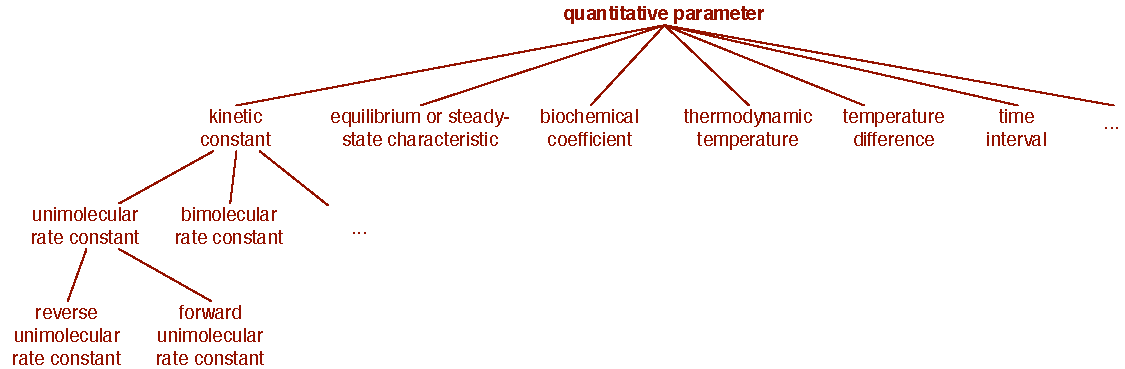
\includegraphics[scale = 0.86]{figs/sbo-quantitative-parameter}
  \caption{Partial expansion of some of the terms in the
    \emph{quantitative parameter} branch.}
  \label{fig:expanded-parameter}
\end{figure}

The terms of the SBO quantitative parameter branch contain
mathematical formulas that are encoded using \mathmltwo; these
formulas define the parameter value using other SBO parameters.
The main use of this approach is to avoid listing all the variants
of a mathematical expression, escaping a combinatorial explosion.

The \emph{modeling framework} controlled vocabulary is needed to
elucidate how to simulate a mathematical expression used in models.
Figure~\vref{fig:expanded-framework} illustrates the structure of
this branch, which is at this point extremely simple, but we
expect that more terms will evolve in the future.

\begin{figure}[tbh]
  \centering
  \vspace{-1ex}
  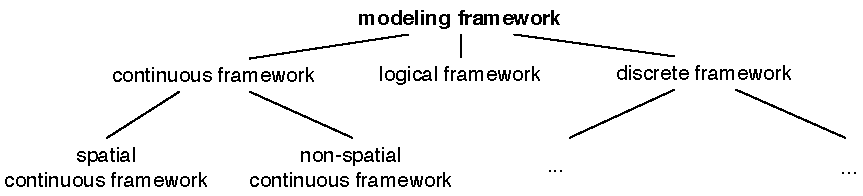
\includegraphics[scale = 0.83]{figs/sbo-framework}
  \caption{Partial expansion of some of the terms in the
    \emph{modeling framework} branch.}
  \label{fig:expanded-framework}
\end{figure}

The \emph{mathematical expression} vocabulary encompasses the
various mathematical expressions that constitute a model.
Figure~\vref{fig:sbo-math-expression} illustrates a portion of the
hierarchy.  Rate law or conservation law formulas are part of the
mathematical expression hierarchy, and subdivided by successively
more refined distinctions until the leaf terms represent precise
statements of common reaction or rule types.  Other types of
mathematical expressions may be included in the future in order to
be able to further characterize mathematical components of a
model, such as initial assignments, assignment rules, rate rules,
algebraic rules, constraints, and event triggers and assignments.

\begin{figure}[tbh]
  \centering
  \vspace*{-1ex}
  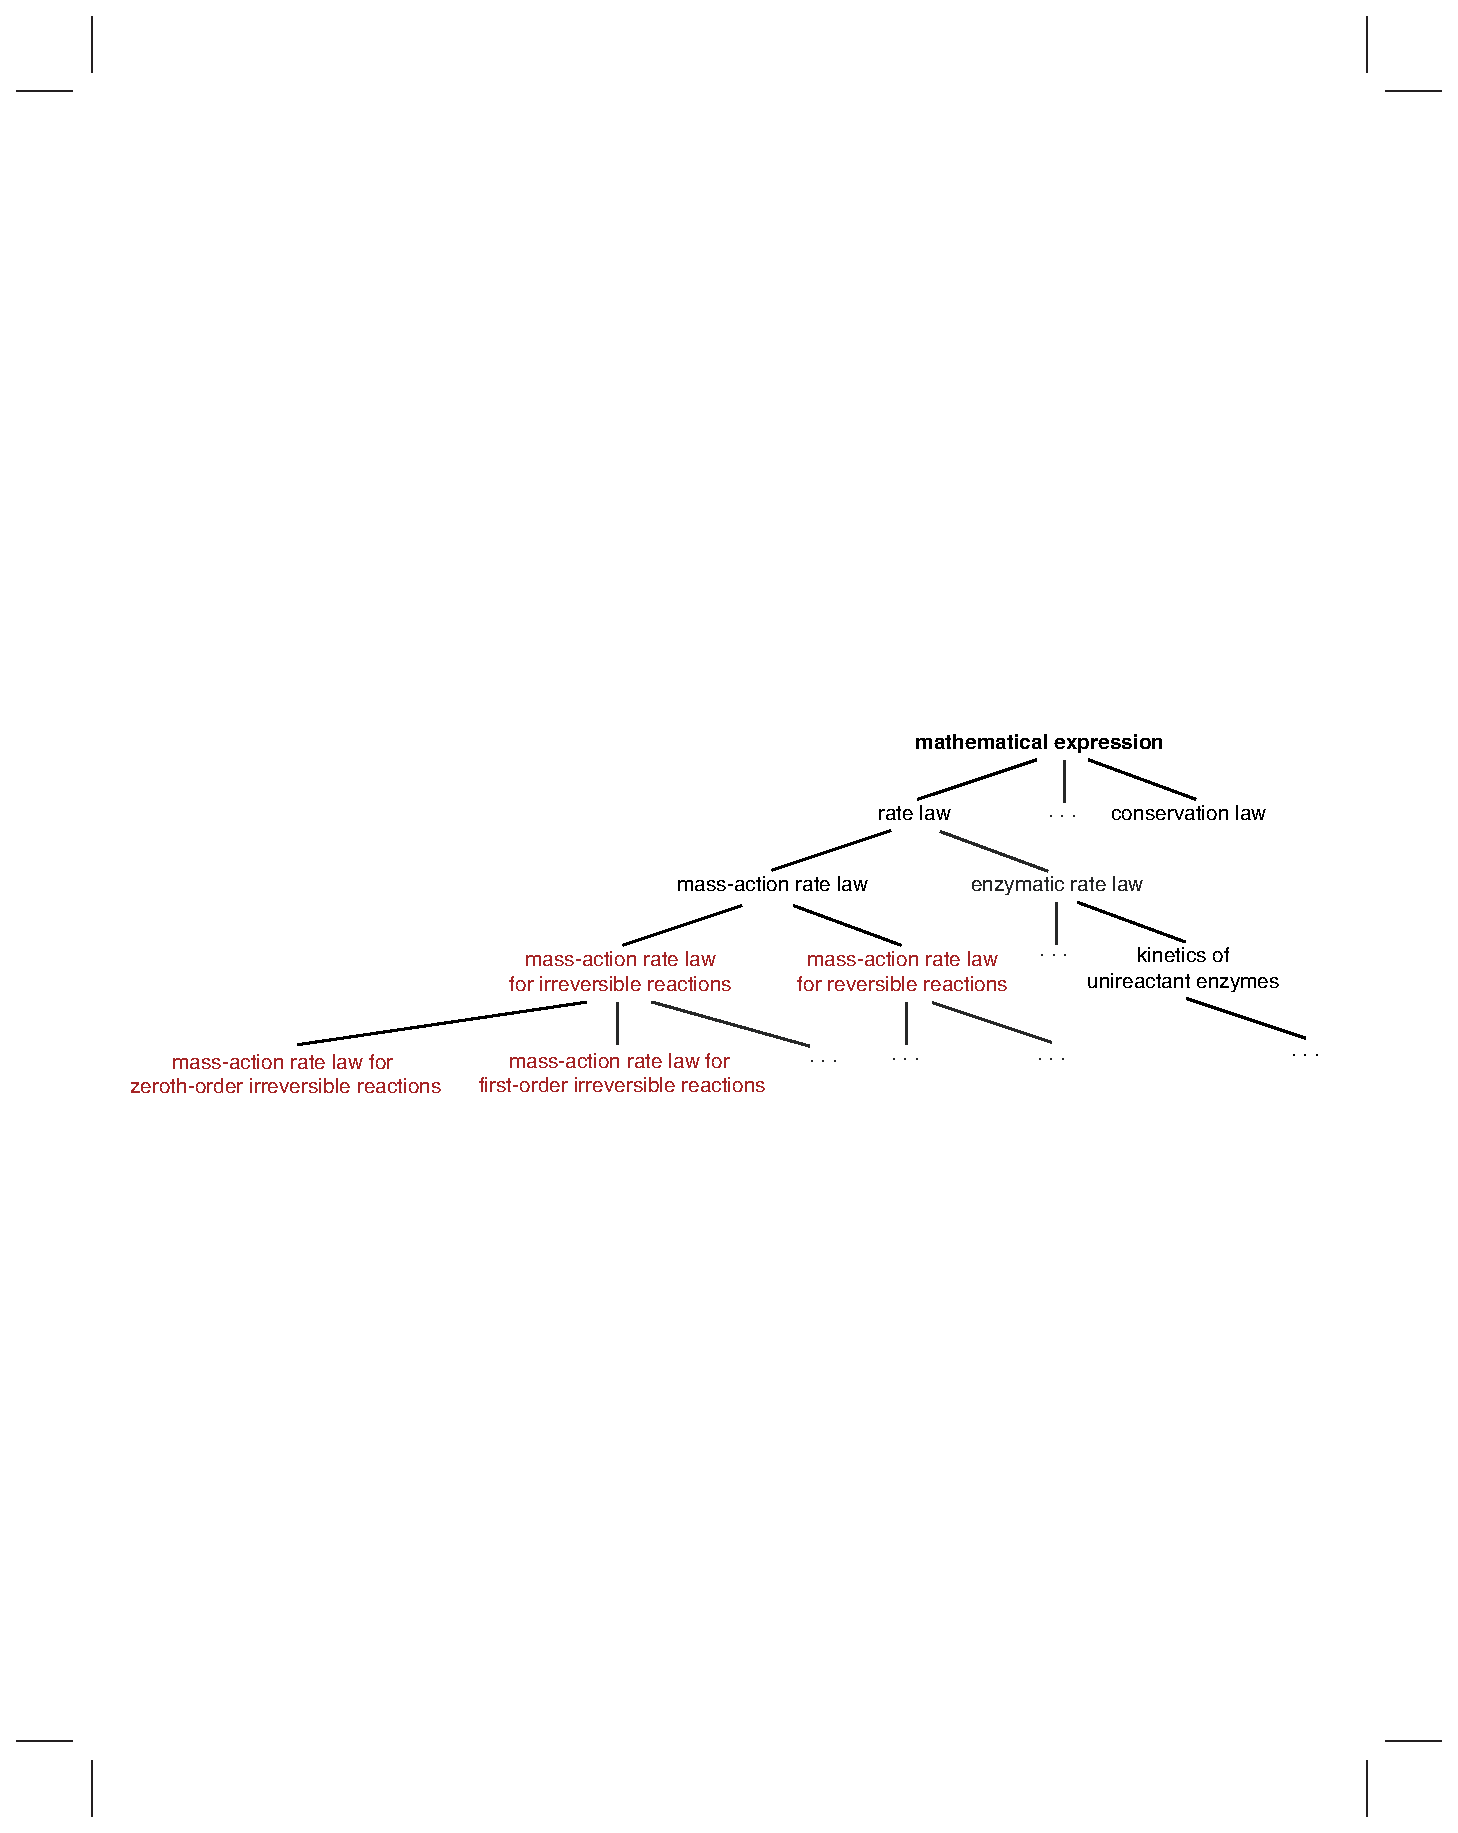
\includegraphics[scale = 0.8, trim=10 0 0 0]{figs/sbo-math-expression}
  \caption{Partial expansion of some of the terms in the \emph{mathematical
      expression} branch.}
  \label{fig:sbo-math-expression}
\end{figure}

The leaf terms of the mathematical expression branch contain the
mathematical formulas encoded using \mathmltwo.  There are many
potential uses for this.  One is to allow a software application
to obtain the formula corresponding to a term and use it as the
basis of an expression to insert into a model.  In effect, the
formulas given in the CV act as templates for what to put into an
SBML construct such as \KineticLaw or \Rule.  The MathML
definition also acts as a precise statement about the rate law in
question. In particular, it carries information about the modeling
framework to use in order to interpret the formula.  Some of the
non-leaf terms also contain formulas encoded using \mathmltwo. In
that case, the formulas contained in the children terms are
specific versions of the formula contained in the parent term.
Those formulas may be generic, containing MathML constructs not
yet supported by SBML, and need to be expanded into the MathML
subset allowed in SBML before they can be used in conjunction with
SBML models.

To make this discussion concrete, here is an example definition of
an entry in the SBO rate law hierarchy at the time of this
writing.  This term represents second-order, irreversible,
mass-action rate laws with one reactant, formulated for use in a
continuous modeling framework:
\begin{description}

\item \emph{ID}: \token{SBO:0000052}

\item \emph{Name}: mass-action rate law for second-order
  irreversible reactions, one reactant, continuous scheme

\item \emph{Definition}: Reaction scheme where the products are
  created from the reactants and the change of a product quantity
  is proportional to the product of reactant activities. The
  reaction scheme does not include any reverse process that
  creates the reactants from the products. The change of a product
  quantity is proportional to the square of one reactant quantity.
  It is to be used in a reaction modeled using a continuous
  framework.

\item \emph{Parent(s)}: \\
  \token{SBO:0000050}: mass-action rate law for second-order
    irreversible reactions, one reactant (\emph{is-a}).
    \\
    \token{SBO:0000163}: mass-action rate law for irreversible
    reactions, continuous sceheme (\emph{is-a}).
  
\item \emph{MathML}:\vspace*{-1ex}
  \begin{example}
<math xmlns="http://www.w3.org/1998/Math/MathML">
   <semantics definitionURL="http://biomodels.net/SBO/#SBO:0000062">
      <lambda>
         <bvar><ci definitionURL="http://biomodels.net/SBO/#SBO:0000036">k</ci></bvar>
         <bvar><ci definitionURL="http://biomodels.net/SBO/#SBO:0000509">R</ci></bvar>
         <apply>
            <times/>
            <ci>k</ci>
            <ci>R</ci>
            <ci>R</ci>
         </apply>
      </lambda>
   </semantics>
</math>
\end{example}

\end{description}

In the MathML definition of the term shown above, the bound
variables in the \token{lambda} expression are tagged with
references to terms in the SBO quantitative parameter
\changed{branch (for \token{k} and \token{R})}.  This makes it
possible for software applications to interpret the intended
meanings of the parameters in the expression.  This also permits
to convert an expression into another, by using the \mathmltwo
formula contained in the SBO terms associated with the parameters.

The \emph{interaction} branch of SBO defines types of biological
processes, events or relationship involving entities.  It lists
the types of biochemical reactions, such as binding,
conformational transition, or cleavage, and also the different
controls that modify a biochemical reaction, such as inhibition,
catalysis, etc.

\begin{figure}[tbh]
  \centering
  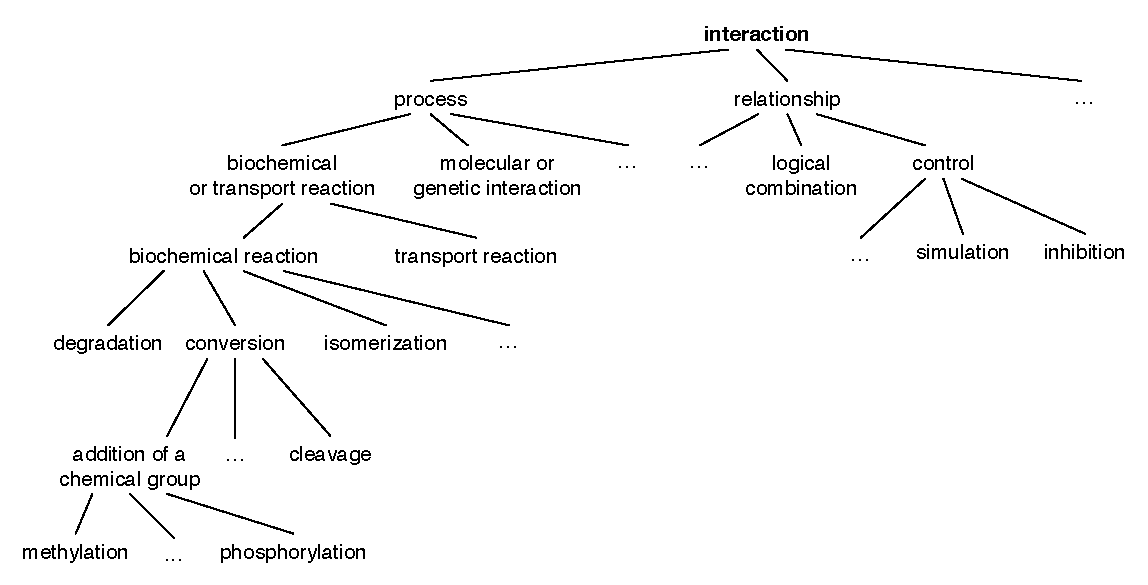
\includegraphics[scale = 0.82]{figs/sbo-interaction}
  \caption{Partial expansion of some of the terms in the \emph{interaction} branch.}
  \label{fig:sbo-interaction}
\end{figure}

One of the goals of SBO is to permit a tool to traverse up and
down the hierarchy in order to find equivalent terms in different
frameworks.  The hope is that when a software tool encounters a
given rate formula in a model, the formula will be a specific form
(say, ``mass-action rate law, second order, one reactant, for
discrete simulation''), but by virtue of the consistent
organization of the reaction rate CV into framework-specific
definitions, and the declaration of every parameters involved in
each expression, the tool should in principle be able to determine
the definitions for other frameworks (say, ``mass-action rate law,
second order, one reactant for \emph{continuous} simulation'').
If the software tool is designed for continuous simulation and it
encounters an SBML model with rate laws formulated for discrete
simulation, it could in principle look up the rate laws'
identifiers in the CV and search for alternative definitions
intended for discrete simulation.  And of course, the converse is
true, for when a tool designed for discrete simulation encounters
a model with rate laws formulated for continuous simulation.


\subsubsection{Relationships between individual SBML components and SBO terms}

The \token{sboTerm} attribute is defined on the abstract class
\SBase and can be used in all derived elements.  However, not all
SBO terms should be used to annotate all SBML elements.
Table~\ref{tab:sboterm-availability} summarizes the relationships
between SBML components and the branches within SBO that apply to
that component. (There are currently no specific SBO term that
correspond to the \SBML, \UnitDefinition, \Unit, and various
\class{ListOf\rule{0.5in}{0.5pt}} list classes.)

\begin{table}[t]
  \small
  \centering
  \begin{tabular}{lll}
    \toprule
    \textbf{SBML Component} & \textbf{SBO Branch} & \textbf{Branch Identifier} \\
    \midrule
    \Model              & interaction			& \sbointeractionID \\
    \FunctionDefinition & mathematical expression   	& \sbomathformulaID \\
    \Compartment        & material entity 		& \sbomaterialentityID \\
    \Species            & material entity 		& \sbomaterialentityID \\
    \Reaction           & interaction     		& \sbointeractionID \\
    \Parameter          & quantitative parameter    	& \sboparameterID \\
    \SpeciesReference   & participant role          	& \sboparticipantroleID \\
    \ModifierSpeciesReference & participant role	& \sboparticipantroleID \\
    \KineticLaw         & rate law                  	& \sboratelawID \\
    \LocalParameter     & quantitative parameter    	& \sboparameterID \\
    \InitialAssignment  & mathematical expression   	& \sbomathformulaID \\
    \AlgebraicRule      & mathematical expression   	& \sbomathformulaID \\
    \AssignmentRule     & mathematical expression   	& \sbomathformulaID \\
    \RateRule           & mathematical expression   	& \sbomathformulaID \\
    \Constraint         & mathematical expression   	& \sbomathformulaID \\
    \Event              & interaction     		& \sbointeractionID \\
    \Trigger            & mathematical expression   	& \sbomathformulaID \\
    \Priority           & mathematical expression   	& \sbomathformulaID \\
    \Delay              & mathematical expression   	& \sbomathformulaID \\
    \EventAssignment    & mathematical expression   	& \sbomathformulaID \\
    \bottomrule
  \end{tabular}
  \caption{SBML components and the main types of SBO terms that
    may be assigned to them.  The identifiers of the highest-level
    SBO terms in each branch are provided for guidance, but actual
    values used for \token{sboTerm} attributes should be more
    specific child terms within these branches.  Note that the
    important aspect here is the set of specific SBO identifiers,
    not the SBO term names, because the names may change as SBO
    continues to evolve. See text for further explanations.} 
  \label{tab:sboterm-availability}
\end{table}

The parent identifiers shown in
Table~\ref{tab:sboterm-availability} are provided for reference.
They are the highest-level terms in their respective branch;
however, these are \emph{not} the terms that would be used to
annotate an element in SBML, because there are more specific terms
underneath the parents shown here.  A software tool should use the
most specific SBO term available for a given concept rather than
using the top-level identifier acting as the root of that
particular vocabulary.

\subsubsection{Tradeoffs in using SBO terms}

The SBO-based approach to annotating SBML components with
controlled terms has the following strengths:
\begin{enumerate}

\item The syntax is minimally intrusive and maximally simple,
  requiring only one string-valued attribute.

\item It supports a significant fraction of what SBML users have wanted
  to do with controlled vocabularies.

\item It does not interfere with any other scheme.  The more
  general annotation-based approach described in
  Section~\ref{sec:annotation-standard} can still be used
  simultaneously in the same model.

\end{enumerate}

The scheme has the following weaknesses:
\begin{enumerate}

\item An object can only have one \token{sboTerm} attribute;
  therefore, it can only be related to a single term in SBO.
  (This also impacts the design of SBO: it must be structured such
  that a class of SBML elements can logically only be associated
  with one class of terms in the ontology.)

\item The only relationship that can be expressed by
  \token{sboTerm} is ``is a''.  It is not possible to represent
  different relationships (known as \emph{verbs} in
  ontology-speak).  This limits what can be expressed using SBO.

\end{enumerate}



The weaknesses are not shared by the annotation scheme described
in Section~\ref{sec:annotation-standard}.  



\subsection{Relationships to the SBML \token{annotation} element}

Another way to provide this information would be to place SBO
terms inside the \SBase \token{annotation} element
(Sections~\ref{sec:sbase} and~\ref{sec:annotation-standard}).
However, in the interest of making the use of SBO in SBML as
interoperable as possible between software tools, the
best-practice recommendation is to place SBO references in the
\token{sboTerm} attribute rather than inside the
\token{annotation} element of an object. If instead the approach
of using \token{annotation} is taken, the qualifiers
(Section~\ref{sec:qualified-dc-annotation}) linking the SBML
element and SBO term should be chosen extremely carefully, since
it will no longer be possible to assume an ``instance to class''
relationship.

Although \token{sboTerm} is just another kind of optional
annotation in SBML, SBO references are separated into
their own attribute on SBML components, both to simplify their use
for software tools and because doing so asserts a stronger and
more focused connection in a more regimented fashion.  SBO
references are intended to allow a modeler to make a statement of
the form ``this object is identical in meaning and intention to
the object defined in the term X of SBO'', and do so in a way
that a \emph{software tool can interpret unambiguously}.

Some software applications may have their own vocabulary of terms
similar in purpose to SBO.  For maximal software interoperability,
the best-practice recommendation in SBML is nonetheless to use SBO
terms in preference to using application-specific annotation
schemes.  Software applications should therefore attempt to
translate their private terms to and from SBO terms when writing
and reading SBML, respectively.


\subsection{Discussion}

Here we discuss some additional points about the SBO-based
approach.

\subsubsection{Frequency of change in the ontology}
\label{sec:sbo-frequency-of-change}

The SBO development approach follows conventional ontology
development approaches in bioinformatics.  One of the principles
being followed is that identifiers and meanings of terms in the
CVs never change and the terms are never deleted.  Where some
terms are deemed obsolete, the introduction of new terms refine or
supersede existing terms, but the existing identifiers are left in
the CV.  Thus, references never end up pointing to nonexistent
entries.  In the case where synonymous terms are merged after
agreement that multiple terms are identical, the term identifiers
are again left in the CV and they still refer to the same concept
as before.  Out-of-date terms cached or hard-coded by an
application remain usable in all cases.  (Moreover,
machine-readable CV encodings and appropriate software design
should render possible the development of API libraries that
automatically map older terms to newer terms as the CVs evolve.)
Therefore, a model is never in danger of ending up with SBO
identifiers that cannot be dereferenced.  If an application finds
an old model with a term \token{SBO:0000065}, it can be assured
that it will be able to find this term in SBO, even if it has been
superseded by other, more preferred terms.


\subsubsection{Consistency of information}

If you have a means of linking (say) a reaction rate formula to a
term in a CV, it is possible to have an inconsistency between the
formula in the SBML model and the one defined for the CV term.
However, this is not a new problem; it arises in other situations
involving SBML models already.  The guideline for these situations
is that the model must be self-contained and stand on its own.
Therefore, in cases where they differ, the definitions in the SBML
model take precedence over the definitions referenced by the CV.
In other words, the model (and its MathML) is authoritative.


\subsubsection{Implications for network access}
\label{sec:sbo-implications-for-network-access}

A software tool does not need to have the ability to access the
network or read the CV every time it encounters a model or
otherwise works with SBML.  Since the SBO will likely stabilize
and change infrequently once a core set of terms is defined,
applications can cache the controlled vocabulary, and not make
network accesses to the master SBO copy unless something forces
them to (\eg detecting a reference in a model to an SBO term that
the application does not recognize).  Applications could have user
preference settings indicating how often the CV definitions should
be refreshed (similar to how modern applications provide a setting
dictating how often they should check for new versions of
themselves).  Simple applications may go further and hard code
references to terms in SBO that have reached stability and
community consensus. SBO is available for download under different
formats (\sboref).  Web services are also available to provide
programmatic access to the ontology.
